% !TEX root = ../thesis.tex
% current project state
% @author Tobias Wulf
%

\section{Stand der Vorarbeiten 0.0.1 18.02.2021}\label{sec:stand-der-vorarbeiten}

Einleitend findet, zur Erörterung der Ziele und Inhalte dieser Arbeit, eine kurze Zusammenfassung der Vorarbeiten statt. Für den Inhalt relevante Aspekte der Vorarbeiten werden im \autoref{ch:grundlagen} näher beleuchtet und erklärt.


Aktuell steht kein magnetisches TMR-Sensor-Array als eigenständiges \gls{ac:ic} zur Verfügung. Im Zuge des Forschungsprojekts Signalverarbeitung für \gls{ac:isar} sind in der \gls{gl:ags} Machbarkeitsstudien \cite{Mehm2019}\cite{Ernsting2020} erbracht worden, die generelle Funktionalitäten und die technische Umsetzung eines magnetischen Sensor-Arrays im Maßstab $1:25$ zeigen.
\newline
So ist als erster Ansatz, das in \autoref{fig:sensor-array-platine-8x8} zu sehende Platinen-Sensor-Array entwickelt worden. Für den Aufbau des Platinen-Sensor-Arrays sind einzelne Winkelsensoren in Sensorbänken angeordnet. Die Messwerterfassung erfolgt über ein Hyperplexing-Verfahren.
Eine Steuerung des Hyperplexings und die weitere Messwertverarbeitung erfolgt mit Hilfe eines Mikrocontrollers.

\begin{figure}[tbph]
	\centering
	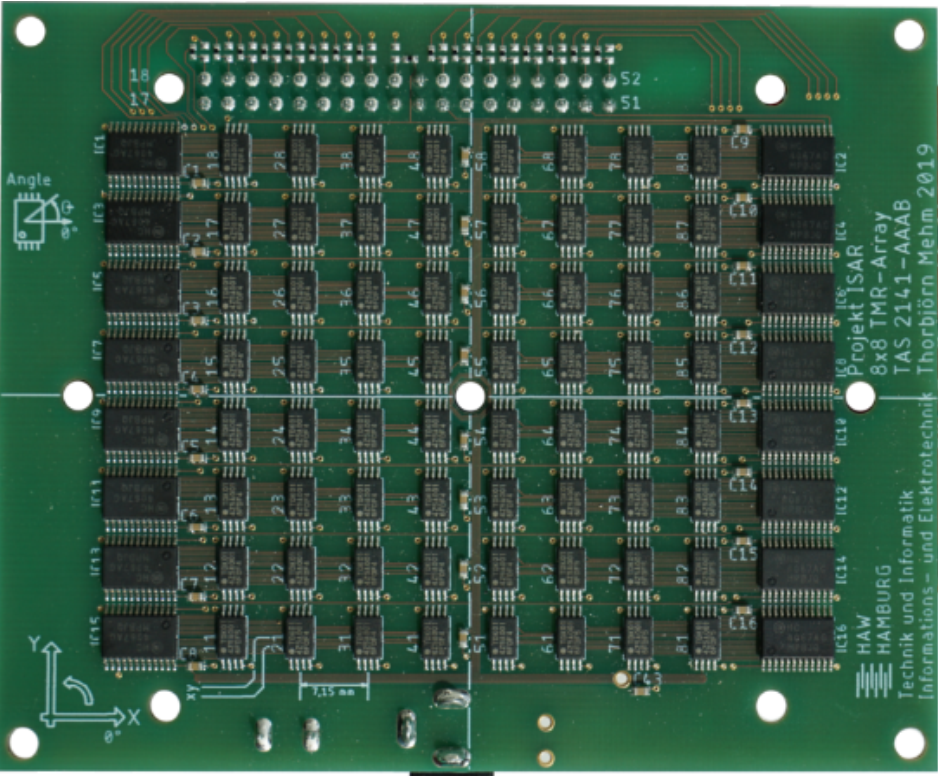
\includegraphics[width=0.7\linewidth]{chapters/images/Sensor-Array-Platine-8x8}
	\caption[Platinen-Sensor-Array Maßstab 1:25]{Platinen-Sensor-Array im Maßstab 1:25 aufgebaut als $8\times8$ Sensor-Array,
		dass als Aufsteckmodul für eine Mikrocontroller getriebene Signalverarbeitung bereitsteht \cite{Mehm2019}.}
	\label{fig:sensor-array-platine-8x8}
\end{figure}

Diese Herangehensweise lässt eine Untersuchung der technischen Machbarkeit auf der Basis von heute zur Verfügung stehenden Technologien und Winkelsensoren zu.
So ist das Platinen-Sensor-Array in verschieden Versionen, mit \gls{ac:amr} Sensoren der Firma NXP Semiconductors (KMZ60) \cite{NXPSemiconductors2014} und TMR Sensoren der Firma TDK (TAS2141-AAAB) \cite{TDK2016} verwirklicht worden. Das Maßstabsmodell des magnetischen Sensor-Arrays kann zu Vergleichs- und weiteren Erprobungsarbeiten genutzt werden, die z.B. Erkenntnisse aus Simulationen und oder Hardware-Optimierungsarbeiten einbinden.

Einen weiteren Ansatz, der durch die \gls{gl:ags} verfolgt wird, ist die Entwicklung eines Simulationsmodells auf Grundlage von Charakterisierungsdatensätzen. Hierfür wird ein einzelnes Sensor-IC, z.B. der TMR Sensor TAS2141-AAAB der Firma TDK, nach einer bestimmten Kennfeldmethode \cite{Schuethe2019} charakterisiert. Der so gewonnene Datensatz kann dann, durch geeignete Interpolationsverfahren, in einer Simulation zur Generierung eines magnetischen Sensor-Arrays genutzt werden.

% Abbildung Simulationsansatz beschreiben und einbinden in drüber liegenden Absastz

\begin{figure}[tbph]
	\centering
	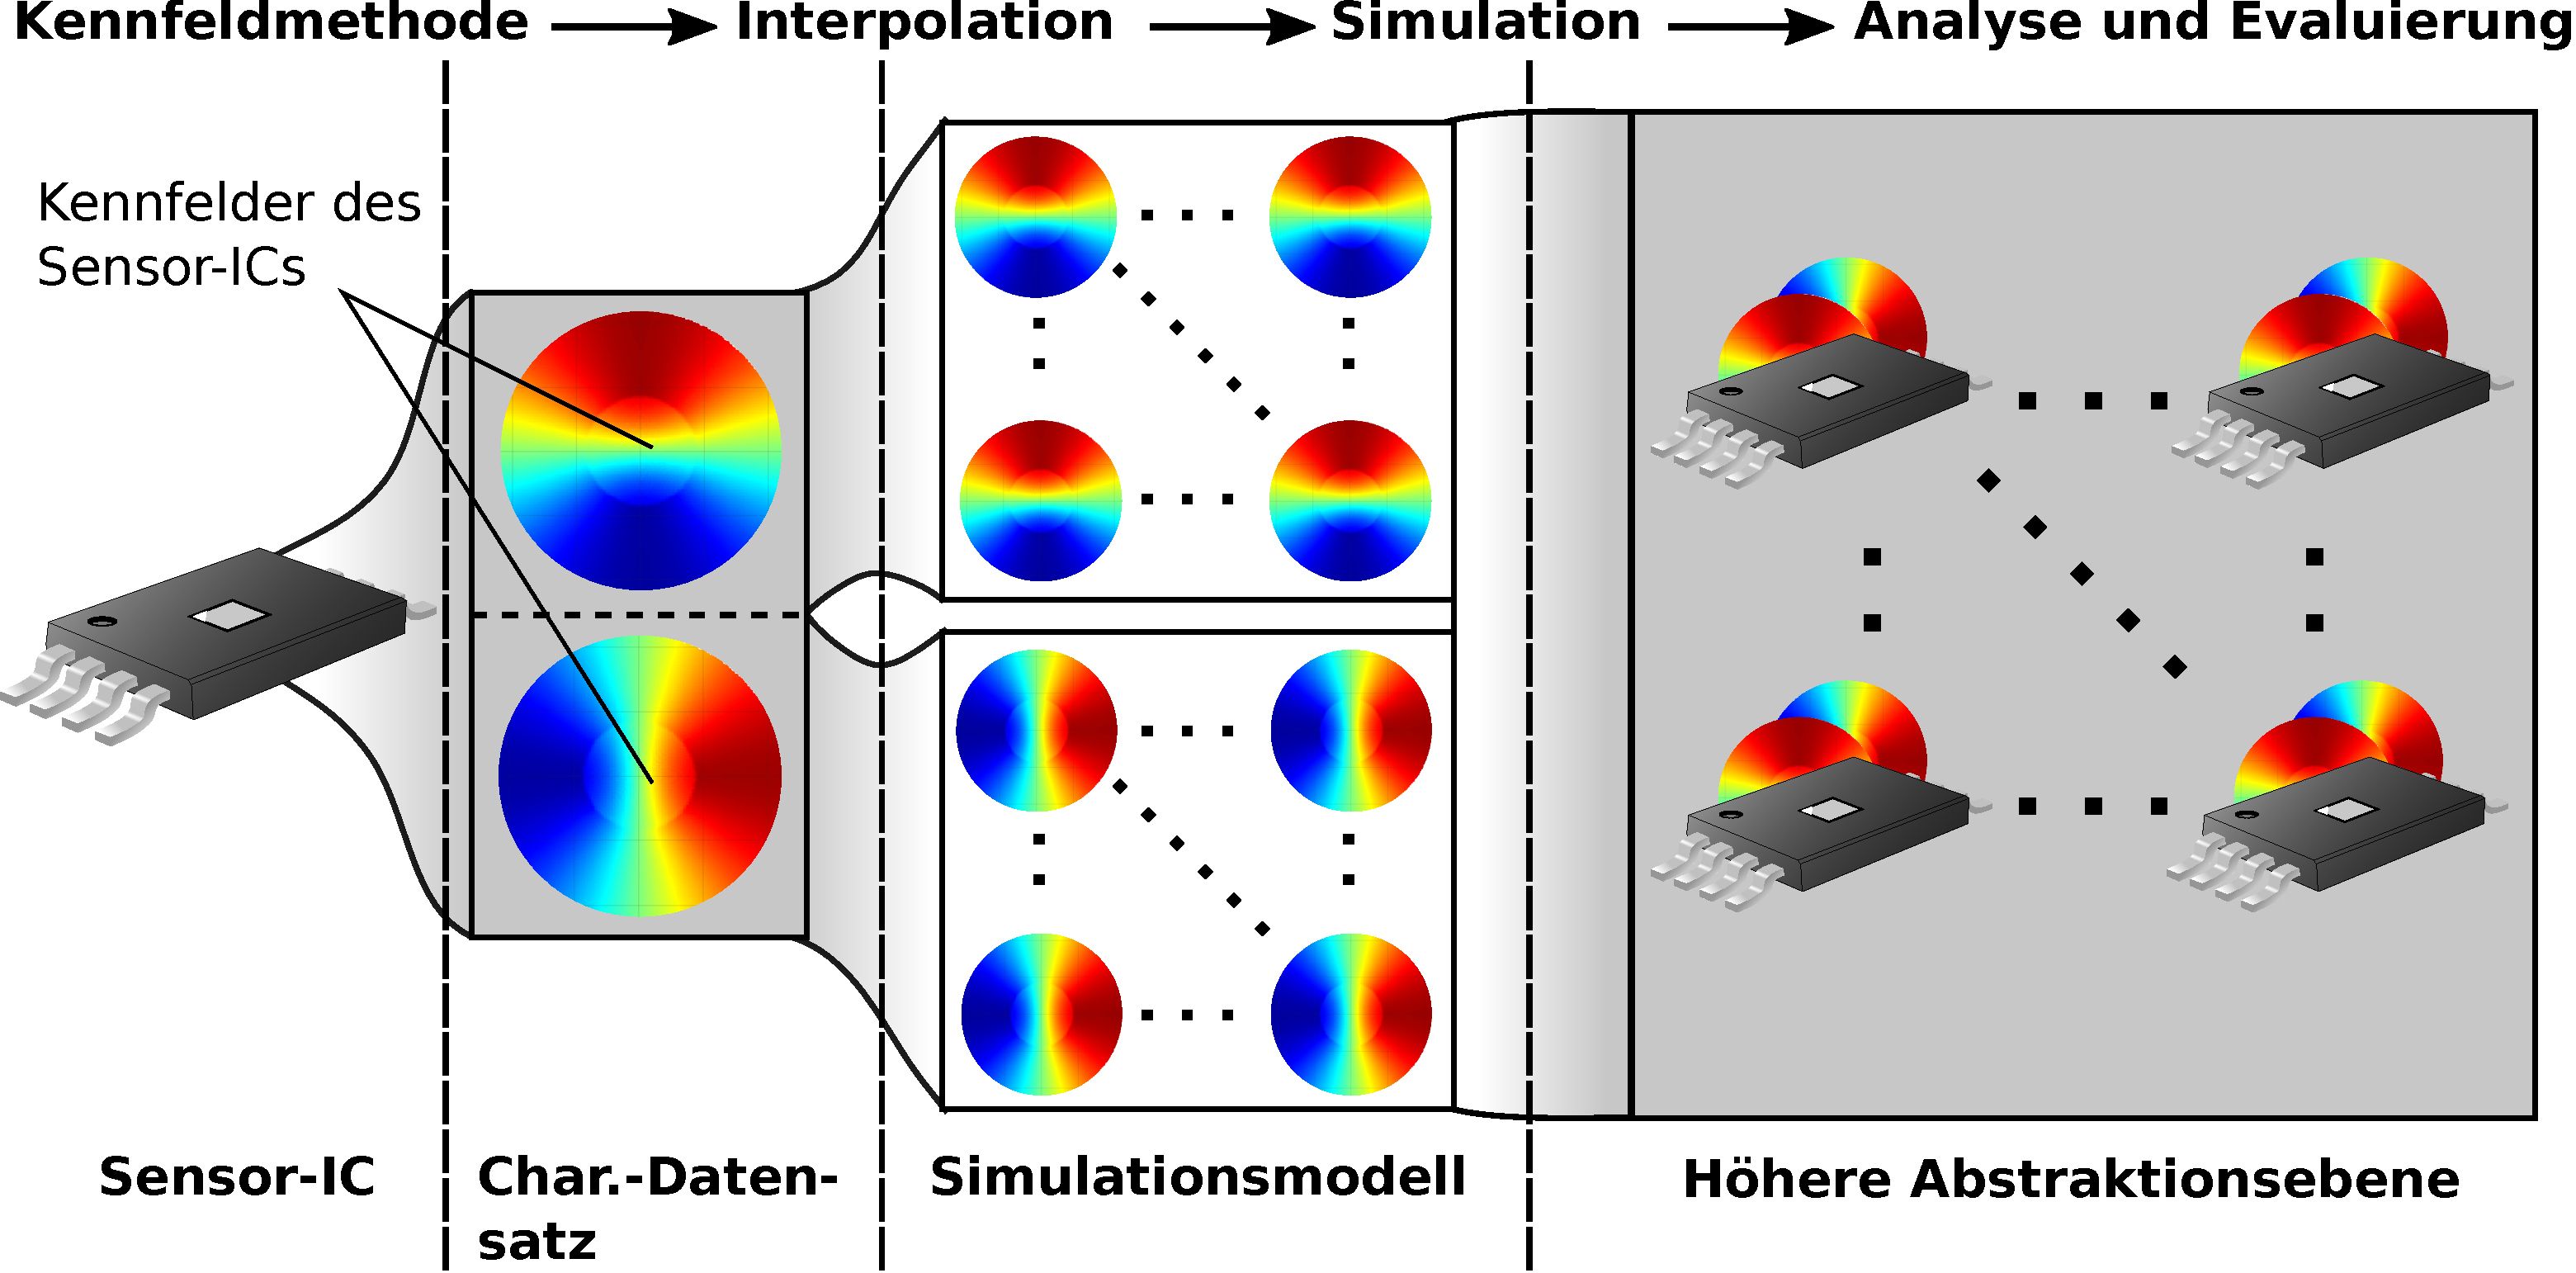
\includegraphics[width=\linewidth]{chapters/images/Ansatz_Simulationsmodell}
	\caption[A]{B}
	\label{fig:ansatzsimulationsmodell}
\end{figure}


